\documentclass[runningheads]{llncs}
\usepackage{graphicx}

\begin{document}
%
\title{Penguin Object Detection Model Development}

\author{Xunyi Zhao}
\institute{University of Tasmania, Newnham TAS 7248, AU}
\authorrunning{X.}
%
\maketitle
%
\begin{abstract}
Penguin, a near-threatened species that live in the southern hemisphere, has been influenced due to the global warming issue recently. The aim of this project is to develop an object detection model, which can detect and classify the type of penguin from images/videos to help Antarctic scientific research. In this project, popular approaches for object detection such as YOLO, R-CNN are used to achieve good performance. On average, the AP50 can reach 87\%+ with the FPS of 70+ by using YOLOv7(w6) model, which is 2.5x times faster and +2\% mmAP more accurate than the best YOLOv5 model(l6) and even more than Faster R-CNN.

\keywords{Antarctica penguins \and Deep learning \and Object detection \and YOLO \and Faster R-CNN \and Model selection.}
\end{abstract}
%
%

% Section 1: Motivation/benefits
\section{Motivation/Benefits}
\subsection{Motivation}
Penguins, a group of aquatic flightless birds, live almost exclusively in the Southern Hemisphere in Antarctica. Among the 20 living species, the \textbf{\textit{Aptenodytes Forsteri (Emperor Penguin)}}, \textbf{\textit{Aptenodytes Patagonicus (King Penguin)}} and \textbf{\textit{Pygoscelis Antarciticus (Chinstrap Penguin)}} are three of the most common and popular species. 

However, due to global warming and other issues, emperor penguins have been identified as Vulnerable or Near Threatened in the latest IUCN Red List~\cite{ref_red_list}. Sometimes, we may find one or two penguins isolated on floating ice (can not find a continent or suitable are for living within 10 kilometres around it).

Thus, I have the motivation to help researchers detect this situation, and also help them to classify the species of penguins automatically, or potentially count the number of penguins in a specific area. Hence, I selected this project and wish to develop an appropriate machine learning application.
\subsection{Real-life benefits}
In real life scenario, this application can detect and then identify the species (only emperor penguins, king penguins and chinstrap penguins due to the time restriction) of penguins living in Antarctica, and count the number of penguins potentially in real-time. What's more, if only one or two penguins are detected within a big area, the system embedded with this model can send the notification, which allows humans to notice this situation quickly and provide corresponding aid if necessary. This will benefit both penguins (ensure population ecological balance) and humans (needn't monitor manually) a lot.


% Section 2: Data collecting
\section{Data collecting}
In this project, nearly all of the data is collected from Google Image~\cite{ref_google_image}. To ensure the quality of the data and helps the model achieve good performance, I have filtered the bad images manually, for example, images with too many penguins, blurry images, low-resolution images etc.

What's more, since the purpose of the application is to detect and then identify the species (and count the number potentially), it is important for me to collect images that contain different numbers of penguins (only 1 penguin or many penguins), clear to see (the higher resolution, the better), and in various context and scenario. Besides, the number of samples and penguin instances should also be large enough, and both penguin adults and chicks (they look pretty different) should be included in the data set. To ensure the quality of the data collecting process, if any situation in the following list happens, then I will not collect that image:

\begin{itemize}
  \item If the image size is too small.
  \item If the image ratio is too weird (say 16:3, which means it's not very square).
  \item If the image contains too many penguins (\textgreater{100}) or is blurry.
  \item If the penguins are drawn by humans.
\end{itemize}

If the image resolution (size) is low, the image will be even more blurry after resizing before/during the training process, so the model could not extract the key features of the image and the performance will be impacted. Also, if the image is too narrow (strange image ratio), then the object will be squeezed/stretched too much after resizing, causing difficulties for the model to recognise these objects. Besides, painting images should not be collected because they have many differences from real penguin images. All these aspects will be discussed and analysed again in the model selection part.

Another step in the data collecting process is data augmentation. Augmentation performs transforms on the existing images to create new variations and increase the number of images in the data set. This ultimately makes models more accurate across a broader range of use cases. 
In the real scenario, the environment we monitor may contain some noise and the exposure of the image/video of the observed environment will be different, which would affect the average performance of the model. To help the model be more resilient to camera artifacts, lighting and camera setting changes, I choose to generate more pictures with different \textbf{noise} (Up to 3\% of pixels) and \textbf{exposure} (Between -15\% and +15\%) by using Roboflow tool~\cite{ref_roboflow}


% Section 3: Data annotating
\section{Data annotating}
To annotate the data that I've collected, I also used Roboflow~\cite{ref_roboflow}. Each type of penguin can be labelled using bounding boxs with different colours within a short time, and the annotation can be exported in various forms (COCO, JSON, TXT etc.) for training different models. The following are the rules I stick with to ensure the quality of the data annotating process:

\begin{itemize}
  \item Make sure the bounding box cover the whole body of each penguin.
  \item If the image contains many penguins, and some of the penguins are too small/blurry/not distinctly visible, just annotate the clear penguins that stand in the front. *
  \item If only the head of the penguin can be seen, make sure to annotate the head.
  \item Annotate the penguin chick as well.
\end{itemize}

* The reason why I ignored some penguins that are too small/blurry/not distinctly visible is that, although as humans, we can know that these "objects" are penguins, if the model learns too much of this "information", it would have some problems such as over-fitting or can not detect the penguins correctly, it will treat any similar blurry things as penguin which is not good for the general case. If the application is used for counting the number of penguins in the image, then I should label all the penguins that I can see. But the main purpose is to detect and classify, thus, to balance this situation and ensure the model has high generalizability, I choose to ignore the blurry penguins in the background.

% Section 4: Data processing
\section{Data processing}
Data processing is a crucial phase in the machine learning process since the quality of the data and the information that can be extracted from it directly influence how well the model can learn. 

A crucial step in computer vision pre-processing is image resizing. The images I collected don't have the same size, although, in some models like YOLOv5, the image resizing is done automatically before training, however, other models like R-CNN will not. Principally, deep learning models train faster on small images. A larger input image requires the neural network to learn from four times as many pixels, which increases the architecture's training time~\cite{resize}. Thus, I choose the resize option in Roboflow~\cite{ref_roboflow} to make sure all the image has the size 640*640.

Usually, an image is captured with metadata that specifies how it should be displayed in relation to how the pixels are arranged on the disc. Most cameras store images' pixels exactly the same whether the camera is oriented in landscape or portrait mode. They just flip a bit to signal to the viewer whether to display the pixels as-is or to rotate them by 90 or 180 degrees when displaying the image. Unfortunately, this can cause issues if the application displaying the images is unaware of the metadata and naively displays the image without respecting its EXIF orientation. Thus, to avoid orientation issues, I choose the Auto-Orient option in Roboflow~\cite{ref_roboflow}.

During the data annotating, I used the scientific name for each type of penguin which is hard for the general user to understand. Thus, to help users know what the species are when the model detects objects, I choose to modify the class name (for example, King Penguin replaces Aptenodytes Patagonicus).

Since the data set does not contain missing values/annotations, I needn't perform any operations on it, and I didn't need to normalize the data as well (which means I keep the original colour as it is). 

After the data collecting and the data processing, there have 1188 images in the data set, and the train/validation/test split I use is 84\%/9\%/7\%.


% Section 5: Model design
\section{Model selection/design}
After processing the data, I need to select and design appropriate approaches (three in total) for this project. 

Among different approaches for object detection tasks, the Region-based Convolutional Neural Network (R-CNN), as a two-step object detection method, is suitable for this project. It separates object detection and recognition into two phase and can apply high-capacity convolutional neural networks (CNNs) to bottom-up region proposals in order to localize and segment objects. When there is a lack of labelled training data, supervised pre-training for a secondary task followed by domain-specific fine-tuning results in a noticeable performance improvement~\cite{R-CNN}. Although R-CNN is slower than the one-step object detection models, it can achieve better average precision potentially. Faster R-CNN, as its name, is the fastest R-CNN. The `region proposal network' (RPN), a component that uses the feature maps generated by a convolutional neural network to suggest a set of bounding boxes where objects may be located, is the main innovation in this system. By incorporating region detection into the primary neural network architecture,Faster R-CNN is able to detect objects quickly and nearly in real time~\cite{Faster R-CNN}.

YOLO, as a one-step object detection model, is the integration of the entire object detection and classification process~\cite{YOLO}. Instead of extracting features and regions separately, YOLO performs everything in a single pass through a single network. In addition, YOLO can perform object detection at video streaming framerates and is suitable application that require real-time inference like this project. YOLO has published 7 different versions by this year, and the most two popular versions are the YOLOv5 and the latest version YOLOv7. The reason why I don't use YOLOv6 is it defines the model parameters directly in Python instead of YAML file, which means it has less customizability than YOLOv5. YOLOv7, on the other hand, is published in August and is 120\% faster than the other versions. In order to compare the difference, I will choose both versions of YOLO. 

There also have several other approaches such as SSD, though it is faster than R-CNN, the performance of it is not as good as R-CNN in some scenarios, and I'm not very familiar with this method, so I didn't choose this as one of my three approaches. Hence, the final three models I choose for this project are YOLOv5, YOLOv7, and Faster R-CNN.

% Section 6: Model selection
\section{Model selection}
% Section 6.1: Metrics and Strategy
\subsection{Selection metrics and strategy}
In this project, I have chosen the following popular metrics to evaluate the models. When selecting the models, we need to consider all the following metrics comprehensively. The ideal model should be both accurate and fast:
\begin{itemize}
  \item IOU (Intersection Over Union): a statistic that determines the distinction (ratio) between anticipated bounding boxes and ground truth annotations. This is the threshold value for the AP and mAP.
  \item AP (Average Precision) and mAP (Mean Average Precision): To evaluate the detection commonly we calculate the area under precision-recall curve, which gives a numerical value that is easy to compare the performance with other models. Based on the precision-recall curve AP, it summarises the weighted mean of precision for each threshold with the increase in recall. Average precision is calculated for each object. However, in AP, we only calculate individual objects but in mAP (the average AP for each class), it gives the precision for the entire model. In this project, I will use AP50, mAP50 (mAP and AP with IOU=0.5, to remove unnecessary bounding boxes, it is the standard threshold value for most of the models), AP@[50:95] (AP) and mAP@[50:95] (mmAP) which are the average of AP and mAP with IOU from 0.5 to 0.95, with the step of 0.05 especially.
  \item FPS (Frames Per Second): I will use FPS to calculate the images/frames the model can detect for each second.
\end{itemize}

In this project, the grid-search strategy is not very suitable due to the time restriction since there may have so many combinations. Instead, we can apply random search manually with the following steps and strategies:
\begin{enumerate}
    \item Generally compares the three main models' performance, if one of them is much worse than the others, filter this one and focus on the better two models.
    \item Train several sub-models of the remaining models (change the pre-trained weights and cfg in YOLO or model in model\_zoo in Faster R-CNN). Compare different sub-models, and choose the best model.
    \item Experiment with different image-size, class-balance, augmentation for this model and decide/train the final best model.
\end{enumerate}


% Section 6.2: Results analysis
\subsection{Results analysis}
According to the model selection strategy and relevant metrics, I trained and performed a general comparison of the YOLOv7, YOLOv5(s), Faster R-CNN models at first. The results can be found in Table~\ref{tab1}. We can see for all of the AP, mAP (mAP50) and mmAP(mAP[50-95]) of YOLOv7 model are apparently higher than the other two models, and it has enough speed (83FPS, nearly catch up YOLOv5s which is one of the fastest models in YOLOv5). This means we must keep YOLOv7 for the later experiment. Faster R-CNN on the other hand has similar performance as YOLOv5s model, but 10 times slower than YOLOv5s. Interestingly, YOLOv5s is one of the worst models in YOLOv5 family, many models like YOLOv5m, YOLOv5l can achieve better performance than it. However, the R-101-FPN model I used for Faster R-CNN is one of the best models in Detectron2 Faster R-CNN family. That means YOLOv5 still have the capacity to become better, but Faster R-CNN hasn't. Thus, I kept the two YOLO models for the later experiment.

% result table
\begin{table}
\centering
\caption{General comparison of three main models}\label{tab1}
\begin{tabular}{|c|c|c|c|c|c|c|}
\hline
\textbf{Model} & \textbf{AP(Chinstrap)} & \textbf{AP(Emperor)} & \textbf{AP(King)} & \textbf{mAP50} & \textbf{mmAP} & \textbf{FPS} \\
\hline
YOLOv7 & \textbf{71.1\%} & \textbf{56.7\%} & \textbf{63.4\%} & \textbf{86.6\%} & \textbf{64.0\%} & 83 \\
YOLOv5s & 62.9\% & 53.2\% & 51.2\% & 82.4\% & 55.8\% & \textbf{92} \\
Faster R-CNN & 65.0\% & 50.4\% & 58.9\% & 82.3\% & 58.1\% & 10\\
\hline
\end{tabular}
\end{table}

After that, I trained different sub-models of YOLO, and the results are listed in Figure~\ref{fig1}. If the specific performance of the model can achieve the top 3/best among all sub-models, I would label them as light/dark green. We can see YOLOv7 and YOLOv5-p6 models perform better than other models, with 86\%+ mAP50 ad 65\%+mmAP on average. Besides, the AP50 of each class are also outstanding, with 82\%+ AP50 for Emperor and King penguins, and 90\%+ for Chinstrap Penguin.

\begin{figure}
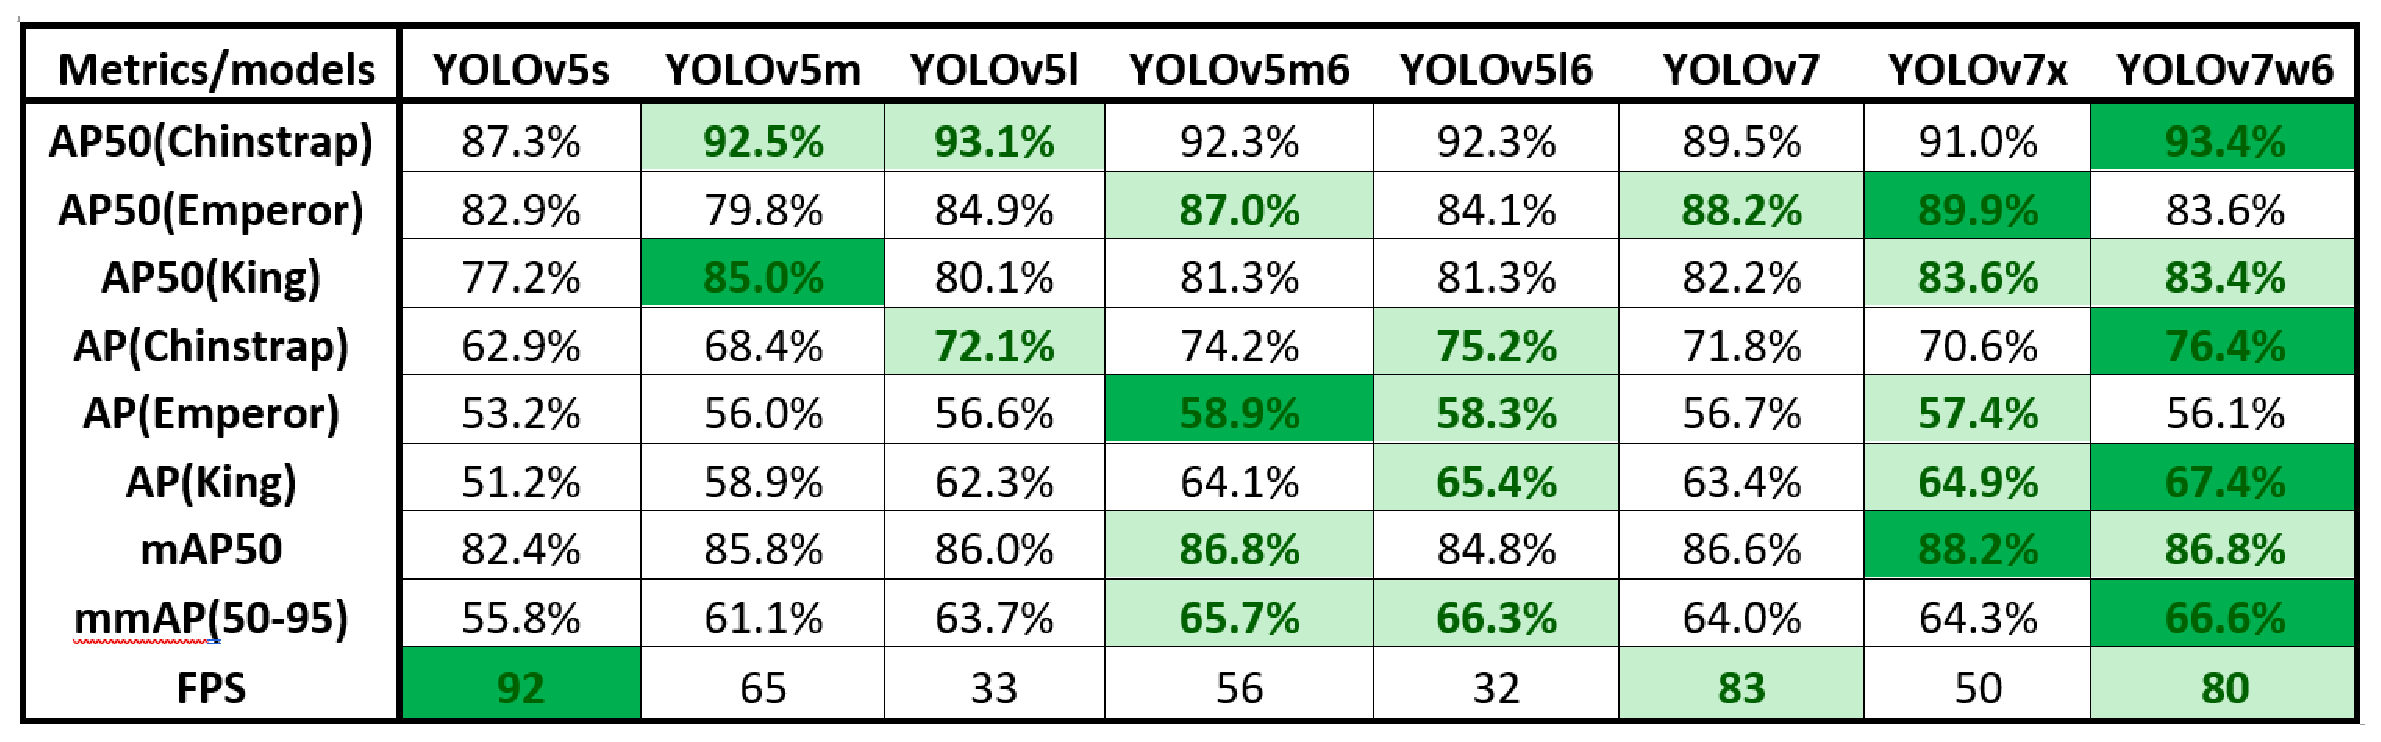
\includegraphics[width=\textwidth]{result.eps}
\caption{Results for sub-models of YOLOv5 and YOLOv7} \label{fig1}
\end{figure}


In the end, I kept the original hyperparameters but tested different image-size, augmentation, batch size etc., to see if they will have impacts on the model. The results are shown in Table~\ref{tab2}. We can see smaller image size has negative impact on the model, but bigger image size doesn't. Besides, as we anticipate, the model can obtain better results if we perform data augmentation and different batch size won't impact the final result a lot (since it will converge to the same point in the end). Hence, I will use 640 as the image size, and batch size 16, and make sure the data is augmented to ensure the model has good performance.
\begin{table}
\centering
\caption{Compare the results (mAP50) with different settings of YOLOv7-w6}\label{tab2}
\begin{tabular}{p{2cm}p{1cm}|p{1.2cm}p{1cm}|p{2cm}p{1cm}}
\hline
\multicolumn{2}{c}{\textbf{Image size}} & \multicolumn{2}{c}{\textbf{Augmentation}} & \multicolumn{2}{c}{\textbf{Batch size}} \\
\hline
Size 640 & 86.8\% &  True & 86.8\% &  Batch 16 & 86.8\% \\
Size 448 & 83.5\% &  False & 82.4\% &  Batch 8 & 87.0\% \\
Size 1280 & 86.0\% &   &  &  Batch 32 & 86.3\% \\
\hline
\end{tabular}
\end{table}

% Section 6.3: Select the best model
\subsection{Select the best model}
Based on the analysis of the results, the best model I select is YOLOv7-w6 (with batch-size 16 and image size 640, need data augmentation) since it has the best mmAP(67\%) and very outstanding mAP(87\%) and AP/AP50 for all three penguin classes (see Figure~\ref{fig1}). Though YOLOv5m6, YOLOv5l6 and YOLOv7x can achieve nearly similar performance, YOLOv7w6 is much faster than them, with FPS of 80 (approximately 2-2.5 times faster).

% Section 7: Apply model
\section{Apply the model}
To apply the selected model in real-life sample, we only need to use the detect.py file in YOLOv7 public repository and put the model name in the `weight' field. The model can detect both image and video sources, which means we can embed it in mobile devices with a camera, and then monitor the environment at real-time speed. However, this is not the best approach since we need to clone YOLOv7 every time. Instead, it's better to develop an appropriate system that can automatically operate the detection using this model.

% Section 8: Post-analysis
\section{Post-analysis}
% Section 8.1: Pros/cons
\subsection{Advantages/disadvantages of the approaches}
In this project, there have many pros and cons of the approaches.

Advantages: The pre-chosen models (YOLO, R-CNN) are very suitable for this task; The images are collected from different resources, and data augmentation is performed appropriately, allowing the model to learn more information in various contexts; Some sub-models like YOLOv5m, YOLOv7X, R101-FPN, are tested and compared together during the model selection process; The images are pre-processed appropriately by resizing and orienting them; The final model I selected, which is YOLOv7 model, are the most efficient object detection model; The tensorboard is used for viewing the training process and results within this project, which helps me compare and select models efficiently; The Roboflow tool is used for all the steps before training, save a large amount of time and helps the model obtain excellent performance potentially. 

Disadvantages: I don't have enough time to train other more powerful sub-models of YOLO and Faster R-CNN such as YOLOv5x, YOLOv7-e6e, X101-FPN etc.; The data is annotated manually in a limited period, which may not be accurate enough; The class instances are not balanced in my dataset, with only 360 chinstrap penguins but 750+ emperor and king penguins; I didn't customize many of the hyperparameters of models, which can impact the performance of the results potentially; The number of samples are still not enough for the model to learn, the generalizability of the model can be increased in the future; The settings of Faster R-CNN may contain errors, causing lower average precision.

% Section 8.2: Improvement 
\subsection{Potential improvement}
To improve the model and make the application into a commercial product, there have several things need to be done. 
\begin{itemize}
    \item More image data including various contexts need to be collected, and both image level and bounding box level of data augmentation techniques (different Hue, Saturation, Cutout, Mosaic) can be applied to help the model learn more information.
    \item More chinstrap penguin images should be collected to make class instances more balance.
    \item More accurate data annotation should be performed, and the annotation should be checked by different developers.
    \item We can customize the hyperparameters or try different sub-versions of YOLOv7 model (YOLOv7-e6e, YOLOv7-D6 etc.), and the model should train for more epochs to obtain even better performance.
    \item The model should be embedded into an appropriate mobile application that can generate/display human-readable statistics and make notifications
\end{itemize}


% Section 8.3: Other approaches
\subsection{Other models/approaches}
In this project, there have some other potential models/approaches that can be used later. For example, the Single Shot MultiBox Detector (SSD) can achieve 72.1\% mAP and 58 FPS~\cite{ssd}, the RetinaNet, the EfficientNet, the MobileNet, the YOLOR etc. Besides, if we can annotate the mask for each penguin, Mask R-CNN is also a good approach for object detection. Fortunately, the final model I used (YOLOv7) is the fastest and one of the most accurate models in the world now, which means all these potential models may not achieve better performance but are still worth trying. 

What's more, better model selection methods such as grid search or fully-random search should be used for obtaining the best hyperparameters combination. Also, we should try to train the same model multiple times and average its results when evaluating the model if possible. 



% Reference
\begin{thebibliography}{8}
\bibitem{ref_red_list}
IUCN 2021, The IUCN Red List of Threatened Species, IUCN Red List of Threatened Species, IUCN.

\bibitem{ref_google_image}
Google Images n.d., Google.com.

\bibitem{ref_roboflow}
Roboflow: Go from Raw Images to a Trained Computer Vision Model in Minutes. n.d., roboflow.ai.

\bibitem{resize}
Saponara, S \& Elhanashi, A 2022, `Impact of Image Resizing on Deep Learning Detectors for Training Time and Model Performance', Lecture Notes in Electrical Engineering, pp. 10–17.

\bibitem{R-CNN}
Girshick, R, Donahue, J, Darrell, T \& Malik, J n.d., Rich feature hierarchies for accurate object detection and semantic segmentation Tech report (v5).

\bibitem{Faster R-CNN}
Ren, S, He, K, Girshick, R \& Sun, J 2015, Faster R-CNN: Towards Real-Time Object Detection with Region Proposal Networks, arXiv.org.

\bibitem{YOLO}
Redmon, J, Divvala, S, Girshick, R \& Farhadi, A 2015, You Only Look Once: Unified, Real-Time Object Detection, arXiv.org.

\bibitem{ssd}
Liu, W, Anguelov, D, Erhan, D, Szegedy, C, Reed, S, Fu, C-Y \& Berg, AC 2016, `SSD: Single Shot MultiBox Detector', Computer Vision – ECCV 2016, pp. 21–37.

\end{thebibliography}
\end{document}
